\documentclass[a4paper,11pt,cours]{nsi} % COMPILE WITH DRAFT
\geometry{margin=2cm}
\usepackage{hyperref}
\usepackage{yhmath}

\begin{document}

\setcounter{chapter}{8} % 1 de moins que le num de chapitre



\chapter{Produit scalaire}


Dans tout le cours, on se place dans un plan muni d'un repère orthonormé $\rep$.
\section{Norme d'un vecteur}

\begin{definition}[]
    Soient $\vv{u}$ un vecteur et deux points $A$ et $B$ tels que $\vv{u} = \vv{AB}$.\\
    On appelle \textbf{norme} de $\vv{u}$ le réel positif ou nul noté $\left\|\vv{u}\right\|$, défini par $\left\|\vv{u}\right\| = AB$.
\end{definition}

\begin{propriete}[]
    Soient $\lambda$ un réel et $\vv{u}$ un vecteur.\\
    On a $\left\|\lambda \vv{u}\right\| = \left|\lambda\right| \times \left\|\vv{u}\right\|$.
\end{propriete}

\begin{propriete}[]
    Dans un repère orthonormé, la norme d'un vecteur $\vc{u}{x}{y}$ est $\left\|\vv{u}\right\| = \sqrt{x^2 + y^2}$.
\end{propriete}

\begin{exemple}[]
    Soient $\pc{A}{-1}{2}$ et $\pc{B}{3}{-1}$.\\[.5em]
    On a $\vc{AB}{3-(-1)}{-1-2}$, donc $\vc{AB}{4}{-3}$.
    \begin{tabbing}
         Ainsi, $\left\|\vv{AB}\right\|$\= $= \sqrt{4^2 + (-3)^2}$\\
         \>$ = \sqrt{16 + 9}$\\
         \>$ = \sqrt{25}$\\
         \>$ = 5$
    \end{tabbing}
\end{exemple}
\newpage

\section{Produit scalaire de deux vecteurs}
Dans cette partie, on considère trois points $A$, $B$ et $C$ et $\vv{u}$ et $\vv{v}$ deux vecteurs non nuls tels que $\vv{u} = \vv{AB}$ et $\vv{v} = \vv{AC}$.\\

\dleft{12cm}{
\begin{definition}[ - Avec des normes seulement (1)]
    Le \textbf{produit scalaire} de $\vv{u}$ et $\vv{v}$ est le réel noté $\vv{u} \cdot \vv{v}$ défini par :
        $$\vv{u} \cdot \vv{v} = \dfrac{1}{2}\left(\left\|\vv{u}\right\|^2+\left\|\vv{v}\right\|^2-\left\|\vv{u}-\vv{v}\right\|^2\right)$$
\end{definition}}
{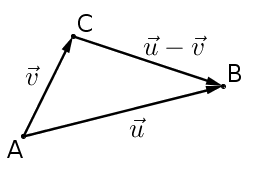
\includegraphics[width=4.5cm]{def.png}}

\dleft{12cm}{
\begin{propriete}[ - Avec des normes seulement (2)]
    $$\vv{u} \cdot \vv{v} =\dfrac{1}{2}\left( \left\|\vv{u}+\vv{v}\right\|^2 - \left\|\vv{u}\right\|^2 - \left\|\vv{v}\right\|^2 \right)$$ 
\end{propriete}}
{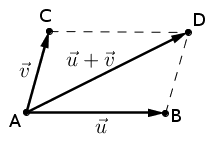
\includegraphics[width=4.5cm]{prop1.png}}

\dleft{12cm}{
\begin{propriete}[ - Avec le projeté orthogonal]
    
\end{propriete}
\end{document}